\documentclass[twoside]{book}

% Packages required by doxygen
\usepackage{fixltx2e}
\usepackage{calc}
\usepackage{doxygen}
\usepackage[export]{adjustbox} % also loads graphicx
\usepackage{graphicx}
\usepackage[utf8]{inputenc}
\usepackage{makeidx}
\usepackage{multicol}
\usepackage{multirow}
\PassOptionsToPackage{warn}{textcomp}
\usepackage{textcomp}
\usepackage[nointegrals]{wasysym}
\usepackage[table]{xcolor}

% Font selection
\usepackage[T1]{fontenc}
\usepackage[scaled=.90]{helvet}
\usepackage{courier}
\usepackage{amssymb}
\usepackage{sectsty}
\renewcommand{\familydefault}{\sfdefault}
\allsectionsfont{%
  \fontseries{bc}\selectfont%
  \color{darkgray}%
}
\renewcommand{\DoxyLabelFont}{%
  \fontseries{bc}\selectfont%
  \color{darkgray}%
}
\newcommand{\+}{\discretionary{\mbox{\scriptsize$\hookleftarrow$}}{}{}}

% Page & text layout
\usepackage{geometry}
\geometry{%
  a4paper,%
  top=2.5cm,%
  bottom=2.5cm,%
  left=2.5cm,%
  right=2.5cm%
}
\tolerance=750
\hfuzz=15pt
\hbadness=750
\setlength{\emergencystretch}{15pt}
\setlength{\parindent}{0cm}
\setlength{\parskip}{3ex plus 2ex minus 2ex}
\makeatletter
\renewcommand{\paragraph}{%
  \@startsection{paragraph}{4}{0ex}{-1.0ex}{1.0ex}{%
    \normalfont\normalsize\bfseries\SS@parafont%
  }%
}
\renewcommand{\subparagraph}{%
  \@startsection{subparagraph}{5}{0ex}{-1.0ex}{1.0ex}{%
    \normalfont\normalsize\bfseries\SS@subparafont%
  }%
}
\makeatother

% Headers & footers
\usepackage{fancyhdr}
\pagestyle{fancyplain}
\fancyhead[LE]{\fancyplain{}{\bfseries\thepage}}
\fancyhead[CE]{\fancyplain{}{}}
\fancyhead[RE]{\fancyplain{}{\bfseries\leftmark}}
\fancyhead[LO]{\fancyplain{}{\bfseries\rightmark}}
\fancyhead[CO]{\fancyplain{}{}}
\fancyhead[RO]{\fancyplain{}{\bfseries\thepage}}
\fancyfoot[LE]{\fancyplain{}{}}
\fancyfoot[CE]{\fancyplain{}{}}
\fancyfoot[RE]{\fancyplain{}{\bfseries\scriptsize Generated by Doxygen }}
\fancyfoot[LO]{\fancyplain{}{\bfseries\scriptsize Generated by Doxygen }}
\fancyfoot[CO]{\fancyplain{}{}}
\fancyfoot[RO]{\fancyplain{}{}}
\renewcommand{\footrulewidth}{0.4pt}
\renewcommand{\chaptermark}[1]{%
  \markboth{#1}{}%
}
\renewcommand{\sectionmark}[1]{%
  \markright{\thesection\ #1}%
}

% Indices & bibliography
\usepackage{natbib}
\usepackage[titles]{tocloft}
\setcounter{tocdepth}{3}
\setcounter{secnumdepth}{5}
\makeindex

% Hyperlinks (required, but should be loaded last)
\usepackage{ifpdf}
\ifpdf
  \usepackage[pdftex,pagebackref=true]{hyperref}
\else
  \usepackage[ps2pdf,pagebackref=true]{hyperref}
\fi
\hypersetup{%
  colorlinks=true,%
  linkcolor=blue,%
  citecolor=blue,%
  unicode%
}

% Custom commands
\newcommand{\clearemptydoublepage}{%
  \newpage{\pagestyle{empty}\cleardoublepage}%
}

\usepackage{caption}
\captionsetup{labelsep=space,justification=centering,font={bf},singlelinecheck=off,skip=4pt,position=top}

%===== C O N T E N T S =====

\begin{document}

% Titlepage & ToC
\hypersetup{pageanchor=false,
             bookmarksnumbered=true,
             pdfencoding=unicode
            }
\pagenumbering{roman}
\begin{titlepage}
\vspace*{7cm}
\begin{center}%
{\Large Motion Controller }\\
\vspace*{1cm}
{\large Generated by Doxygen 1.8.11}\\
\end{center}
\end{titlepage}
\clearemptydoublepage
\tableofcontents
\clearemptydoublepage
\pagenumbering{arabic}
\hypersetup{pageanchor=true}

%--- Begin generated contents ---
\chapter{Motion Controller package}
\label{md_README}
\hypertarget{md_README}{}
\begin{quote}
The package controls a holonomic robot in 2D space by assigning random coordinates and the proper linear velocity to reach them. \end{quote}


\subsection*{Service node}

The service node {\ttfamily /target\+\_\+service} creates the service server {\ttfamily /target} that provides random x and y coordinates. It relies on a custom service message {\ttfamily motion\+\_\+controller/\+Random}.

\subsection*{Random service}

Custom service /\+Random requests {\ttfamily float32 min} and {\ttfamily float32 max} interval values and responds with {\ttfamily float32 x} and {\ttfamily float32 y}.

\subsection*{Controller node}

The node {\ttfamily /motion\+\_\+controller} is subscribed to {\ttfamily /odom} topic, which publishes the robot\textquotesingle{}s current coordinates. The callback function compares these coordinates to the random assigned target and calls the service server {\ttfamily /target} to get a new target if the difference is below a threshold of 0.\+1, otherwise the appropriate linear velocities for x and y are calculated and in turn published to the topic {\ttfamily /cmd\+\_\+vel}.

\subsection*{Nodes Graph}



\subsection*{How to run}

download this folder in your working space\+:


\begin{DoxyCode}
1 git clone kghyfnytfn
\end{DoxyCode}
 build it with {\ttfamily catkin\+\_\+make}, then run the following nodes\+:


\begin{DoxyCode}
1 rosrun stage\_ros stageros $(rospack find assignment1)/wor/exercise.world
2 rosrun motion\_controller target\_service 
3 rosrun motion\_controller motion\_controller 
\end{DoxyCode}
 
\chapter{Class Index}
\section{Class List}
Here are the classes, structs, unions and interfaces with brief descriptions\+:\begin{DoxyCompactList}
\item\contentsline{section}{\hyperlink{structcoord}{coord} }{\pageref{structcoord}}{}
\end{DoxyCompactList}

\chapter{File Index}
\section{File List}
Here is a list of all files with brief descriptions\+:\begin{DoxyCompactList}
\item\contentsline{section}{src/\hyperlink{motion__controller_8cpp}{motion\+\_\+controller.\+cpp} }{\pageref{motion__controller_8cpp}}{}
\item\contentsline{section}{src/\hyperlink{target__service_8cpp}{target\+\_\+service.\+cpp} }{\pageref{target__service_8cpp}}{}
\end{DoxyCompactList}

\chapter{Class Documentation}
\hypertarget{structcoord}{}\section{coord Struct Reference}
\label{structcoord}\index{coord@{coord}}
\subsection*{Public Attributes}
\begin{DoxyCompactItemize}
\item 
float \hyperlink{structcoord_a6b6f43b5ea14a9822f537dc535293036}{x}
\item 
float \hyperlink{structcoord_ad2aee0228903d1f8874a7a43e9227749}{y}
\end{DoxyCompactItemize}


\subsection{Detailed Description}
struct targ containes the variables of the random coordinates assiged in real time 

\subsection{Member Data Documentation}
\index{coord@{coord}!x@{x}}
\index{x@{x}!coord@{coord}}
\subsubsection[{\texorpdfstring{x}{x}}]{\setlength{\rightskip}{0pt plus 5cm}float coord\+::x}\hypertarget{structcoord_a6b6f43b5ea14a9822f537dc535293036}{}\label{structcoord_a6b6f43b5ea14a9822f537dc535293036}
\index{coord@{coord}!y@{y}}
\index{y@{y}!coord@{coord}}
\subsubsection[{\texorpdfstring{y}{y}}]{\setlength{\rightskip}{0pt plus 5cm}float coord\+::y}\hypertarget{structcoord_ad2aee0228903d1f8874a7a43e9227749}{}\label{structcoord_ad2aee0228903d1f8874a7a43e9227749}


The documentation for this struct was generated from the following file\+:\begin{DoxyCompactItemize}
\item 
src/\hyperlink{motion__controller_8cpp}{motion\+\_\+controller.\+cpp}\end{DoxyCompactItemize}

\chapter{File Documentation}
\hypertarget{_r_e_a_d_m_e_8md}{}\section{R\+E\+A\+D\+M\+E.\+md File Reference}
\label{_r_e_a_d_m_e_8md}\index{R\+E\+A\+D\+M\+E.\+md@{R\+E\+A\+D\+M\+E.\+md}}

\hypertarget{motion__controller_8cpp}{}\section{src/motion\+\_\+controller.cpp File Reference}
\label{motion__controller_8cpp}\index{src/motion\+\_\+controller.\+cpp@{src/motion\+\_\+controller.\+cpp}}
{\ttfamily \#include \char`\"{}ros/ros.\+h\char`\"{}}\\*
{\ttfamily \#include \char`\"{}geometry\+\_\+msgs/\+Twist.\+h\char`\"{}}\\*
{\ttfamily \#include \char`\"{}nav\+\_\+msgs/\+Odometry.\+h\char`\"{}}\\*
{\ttfamily \#include \char`\"{}motion\+\_\+controller/\+Random.\+h\char`\"{}}\\*
{\ttfamily \#include \char`\"{}math.\+h\char`\"{}}\\*
Include dependency graph for motion\+\_\+controller.\+cpp\+:\nopagebreak
\begin{figure}[H]
\begin{center}
\leavevmode
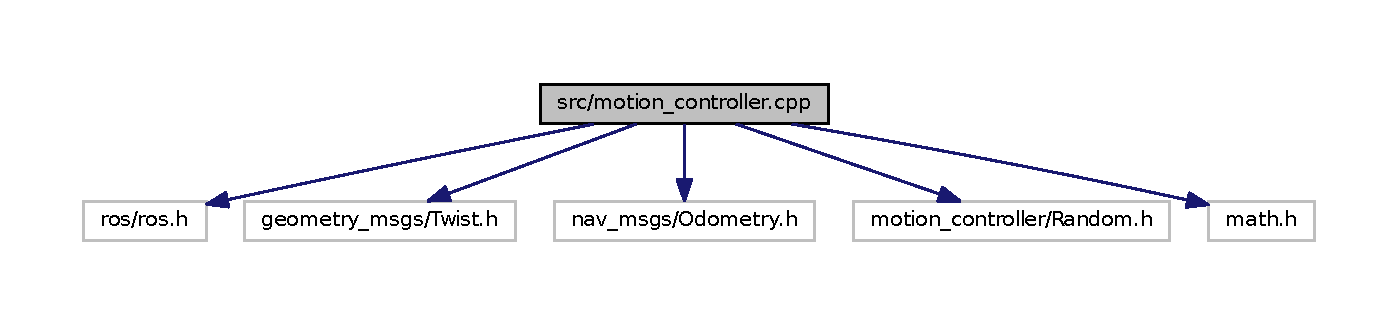
\includegraphics[width=350pt]{motion__controller_8cpp__incl}
\end{center}
\end{figure}
\subsection*{Classes}
\begin{DoxyCompactItemize}
\item 
struct \hyperlink{structcoord}{coord}
\end{DoxyCompactItemize}
\subsection*{Macros}
\begin{DoxyCompactItemize}
\item 
\#define \hyperlink{motion__controller_8cpp_a92ac017207defd4cbfa24eefe0c6236e}{threshold}~0.\+1
\item 
\#define \hyperlink{motion__controller_8cpp_a13b230ea1d237595fb236c951a0849e0}{k}~1
\end{DoxyCompactItemize}
\subsection*{Functions}
\begin{DoxyCompactItemize}
\item 
void \hyperlink{motion__controller_8cpp_aab6e381bffc34921244a29ec0538ba64}{position\+Callback} (const nav\+\_\+msgs\+::\+Odometry\+::\+Const\+Ptr \&msg)
\item 
int \hyperlink{motion__controller_8cpp_a3c04138a5bfe5d72780bb7e82a18e627}{main} (int argc, char $\ast$$\ast$argv)
\end{DoxyCompactItemize}
\subsection*{Variables}
\begin{DoxyCompactItemize}
\item 
struct \hyperlink{structcoord}{coord} \hyperlink{motion__controller_8cpp_a74e01c21daa2619ee6ab2d3b98dd7e09}{targ}
\item 
ros\+::\+Publisher \hyperlink{motion__controller_8cpp_a350594df3e8f6948c8462edfd41ce086}{pub}
\item 
ros\+::\+Service\+Client \hyperlink{motion__controller_8cpp_a17bcd065930a8a7f9f194078d9977268}{client}
\item 
motion\+\_\+controller\+::\+Random \hyperlink{motion__controller_8cpp_ae5e0991bd90659a6d5d475ad208a5d9c}{trg}
\end{DoxyCompactItemize}


\subsection{Macro Definition Documentation}
\index{motion\+\_\+controller.\+cpp@{motion\+\_\+controller.\+cpp}!k@{k}}
\index{k@{k}!motion\+\_\+controller.\+cpp@{motion\+\_\+controller.\+cpp}}
\subsubsection[{\texorpdfstring{k}{k}}]{\setlength{\rightskip}{0pt plus 5cm}\#define k~1}\hypertarget{motion__controller_8cpp_a13b230ea1d237595fb236c951a0849e0}{}\label{motion__controller_8cpp_a13b230ea1d237595fb236c951a0849e0}
\index{motion\+\_\+controller.\+cpp@{motion\+\_\+controller.\+cpp}!threshold@{threshold}}
\index{threshold@{threshold}!motion\+\_\+controller.\+cpp@{motion\+\_\+controller.\+cpp}}
\subsubsection[{\texorpdfstring{threshold}{threshold}}]{\setlength{\rightskip}{0pt plus 5cm}\#define threshold~0.\+1}\hypertarget{motion__controller_8cpp_a92ac017207defd4cbfa24eefe0c6236e}{}\label{motion__controller_8cpp_a92ac017207defd4cbfa24eefe0c6236e}


\subsection{Function Documentation}
\index{motion\+\_\+controller.\+cpp@{motion\+\_\+controller.\+cpp}!main@{main}}
\index{main@{main}!motion\+\_\+controller.\+cpp@{motion\+\_\+controller.\+cpp}}
\subsubsection[{\texorpdfstring{main(int argc, char $\ast$$\ast$argv)}{main(int argc, char **argv)}}]{\setlength{\rightskip}{0pt plus 5cm}int main (
\begin{DoxyParamCaption}
\item[{int}]{argc, }
\item[{char $\ast$$\ast$}]{argv}
\end{DoxyParamCaption}
)}\hypertarget{motion__controller_8cpp_a3c04138a5bfe5d72780bb7e82a18e627}{}\label{motion__controller_8cpp_a3c04138a5bfe5d72780bb7e82a18e627}
\index{motion\+\_\+controller.\+cpp@{motion\+\_\+controller.\+cpp}!position\+Callback@{position\+Callback}}
\index{position\+Callback@{position\+Callback}!motion\+\_\+controller.\+cpp@{motion\+\_\+controller.\+cpp}}
\subsubsection[{\texorpdfstring{position\+Callback(const nav\+\_\+msgs\+::\+Odometry\+::\+Const\+Ptr \&msg)}{positionCallback(const nav_msgs::Odometry::ConstPtr &msg)}}]{\setlength{\rightskip}{0pt plus 5cm}void position\+Callback (
\begin{DoxyParamCaption}
\item[{const nav\+\_\+msgs\+::\+Odometry\+::\+Const\+Ptr \&}]{msg}
\end{DoxyParamCaption}
)}\hypertarget{motion__controller_8cpp_aab6e381bffc34921244a29ec0538ba64}{}\label{motion__controller_8cpp_aab6e381bffc34921244a29ec0538ba64}
The callback function compares the current coordinates published by /odom with nav\+\_\+msgs\+::\+Odometry message type to the target coordinates stored in the struct coord. If the difference is less than the threshold the server /target is called and new target coordinates as stored in targ.\+x and targ.\+y. Otherwise it is calculated the linear velocity to publish on /cmd\+\_\+vel in function of the current position.

N.\+B. In the firs cycle the robot\textquotesingle{}s current position is (0,0) and the target coordinates variables are also initialized as x=0 and y=0, so the first iteration will call the /target service. 

\subsection{Variable Documentation}
\index{motion\+\_\+controller.\+cpp@{motion\+\_\+controller.\+cpp}!client@{client}}
\index{client@{client}!motion\+\_\+controller.\+cpp@{motion\+\_\+controller.\+cpp}}
\subsubsection[{\texorpdfstring{client}{client}}]{\setlength{\rightskip}{0pt plus 5cm}ros\+::\+Service\+Client client}\hypertarget{motion__controller_8cpp_a17bcd065930a8a7f9f194078d9977268}{}\label{motion__controller_8cpp_a17bcd065930a8a7f9f194078d9977268}
\index{motion\+\_\+controller.\+cpp@{motion\+\_\+controller.\+cpp}!pub@{pub}}
\index{pub@{pub}!motion\+\_\+controller.\+cpp@{motion\+\_\+controller.\+cpp}}
\subsubsection[{\texorpdfstring{pub}{pub}}]{\setlength{\rightskip}{0pt plus 5cm}ros\+::\+Publisher pub}\hypertarget{motion__controller_8cpp_a350594df3e8f6948c8462edfd41ce086}{}\label{motion__controller_8cpp_a350594df3e8f6948c8462edfd41ce086}
\index{motion\+\_\+controller.\+cpp@{motion\+\_\+controller.\+cpp}!targ@{targ}}
\index{targ@{targ}!motion\+\_\+controller.\+cpp@{motion\+\_\+controller.\+cpp}}
\subsubsection[{\texorpdfstring{targ}{targ}}]{\setlength{\rightskip}{0pt plus 5cm}struct {\bf coord}  targ}\hypertarget{motion__controller_8cpp_a74e01c21daa2619ee6ab2d3b98dd7e09}{}\label{motion__controller_8cpp_a74e01c21daa2619ee6ab2d3b98dd7e09}
\index{motion\+\_\+controller.\+cpp@{motion\+\_\+controller.\+cpp}!trg@{trg}}
\index{trg@{trg}!motion\+\_\+controller.\+cpp@{motion\+\_\+controller.\+cpp}}
\subsubsection[{\texorpdfstring{trg}{trg}}]{\setlength{\rightskip}{0pt plus 5cm}motion\+\_\+controller\+::\+Random trg}\hypertarget{motion__controller_8cpp_ae5e0991bd90659a6d5d475ad208a5d9c}{}\label{motion__controller_8cpp_ae5e0991bd90659a6d5d475ad208a5d9c}

\hypertarget{target__service_8cpp}{}\section{src/target\+\_\+service.cpp File Reference}
\label{target__service_8cpp}\index{src/target\+\_\+service.\+cpp@{src/target\+\_\+service.\+cpp}}
{\ttfamily \#include \char`\"{}ros/ros.\+h\char`\"{}}\\*
{\ttfamily \#include \char`\"{}motion\+\_\+controller/\+Random.\+h\char`\"{}}\\*
Include dependency graph for target\+\_\+service.\+cpp\+:\nopagebreak
\begin{figure}[H]
\begin{center}
\leavevmode
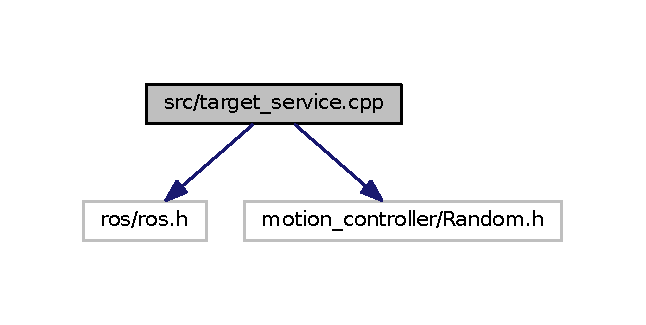
\includegraphics[width=310pt]{target__service_8cpp__incl}
\end{center}
\end{figure}
\subsection*{Functions}
\begin{DoxyCompactItemize}
\item 
double \hyperlink{target__service_8cpp_a10f83119b77a8fbd085a5550955f85ff}{rand\+M\+ToN} (double M, double N)
\item 
bool \hyperlink{target__service_8cpp_a5daf14ef7a24a03f723910e5b3970361}{Callback} (motion\+\_\+controller\+::\+Random\+::\+Request \&req, motion\+\_\+controller\+::\+Random\+::\+Response \&res)
\item 
int \hyperlink{target__service_8cpp_a3c04138a5bfe5d72780bb7e82a18e627}{main} (int argc, char $\ast$$\ast$argv)
\end{DoxyCompactItemize}


\subsection{Function Documentation}
\index{target\+\_\+service.\+cpp@{target\+\_\+service.\+cpp}!Callback@{Callback}}
\index{Callback@{Callback}!target\+\_\+service.\+cpp@{target\+\_\+service.\+cpp}}
\subsubsection[{\texorpdfstring{Callback(motion\+\_\+controller\+::\+Random\+::\+Request \&req, motion\+\_\+controller\+::\+Random\+::\+Response \&res)}{Callback(motion_controller::Random::Request &req, motion_controller::Random::Response &res)}}]{\setlength{\rightskip}{0pt plus 5cm}bool Callback (
\begin{DoxyParamCaption}
\item[{motion\+\_\+controller\+::\+Random\+::\+Request \&}]{req, }
\item[{motion\+\_\+controller\+::\+Random\+::\+Response \&}]{res}
\end{DoxyParamCaption}
)}\hypertarget{target__service_8cpp_a5daf14ef7a24a03f723910e5b3970361}{}\label{target__service_8cpp_a5daf14ef7a24a03f723910e5b3970361}
The callback funtion assigns a random value to the variables x and y between the values min and max every time the service server /target is called. \index{target\+\_\+service.\+cpp@{target\+\_\+service.\+cpp}!main@{main}}
\index{main@{main}!target\+\_\+service.\+cpp@{target\+\_\+service.\+cpp}}
\subsubsection[{\texorpdfstring{main(int argc, char $\ast$$\ast$argv)}{main(int argc, char **argv)}}]{\setlength{\rightskip}{0pt plus 5cm}int main (
\begin{DoxyParamCaption}
\item[{int}]{argc, }
\item[{char $\ast$$\ast$}]{argv}
\end{DoxyParamCaption}
)}\hypertarget{target__service_8cpp_a3c04138a5bfe5d72780bb7e82a18e627}{}\label{target__service_8cpp_a3c04138a5bfe5d72780bb7e82a18e627}
\index{target\+\_\+service.\+cpp@{target\+\_\+service.\+cpp}!rand\+M\+ToN@{rand\+M\+ToN}}
\index{rand\+M\+ToN@{rand\+M\+ToN}!target\+\_\+service.\+cpp@{target\+\_\+service.\+cpp}}
\subsubsection[{\texorpdfstring{rand\+M\+To\+N(double M, double N)}{randMToN(double M, double N)}}]{\setlength{\rightskip}{0pt plus 5cm}double rand\+M\+ToN (
\begin{DoxyParamCaption}
\item[{double}]{M, }
\item[{double}]{N}
\end{DoxyParamCaption}
)}\hypertarget{target__service_8cpp_a10f83119b77a8fbd085a5550955f85ff}{}\label{target__service_8cpp_a10f83119b77a8fbd085a5550955f85ff}
Function that returns a random value between M and N M\+: minimum value N\+: maximum value 
%--- End generated contents ---

% Index
\backmatter
\newpage
\phantomsection
\clearemptydoublepage
\addcontentsline{toc}{chapter}{Index}
\printindex

\end{document}
